%!TEX program = xelatex
% 數論（一）期末口頭報告投影片（約 40 分鐘）
% 重點：LWE 與 Ring-LWE；前置六頁簡介；末段 5 分鐘應用與開放問題
\documentclass[aspectratio=169, 11pt]{beamer}

\usepackage{fontspec}
\usepackage{xeCJK}
\setCJKmainfont{Microsoft JhengHei}
\setmainfont{Times New Roman}

\usepackage{amsmath}
\usepackage{amssymb}
\usepackage{tikz}
\usetikzlibrary{calc, arrows.meta}

% ── 配色與佈景 ─────────────────────────────────────────────
\definecolor{accent}{RGB}{30, 80, 160}
\definecolor{accentlt}{RGB}{237, 246, 255}
\definecolor{warn}{RGB}{200, 90, 30}

\usetheme{default}
\setbeamercolor{structure}{fg=accent}
\setbeamercolor{title}{fg=accent}
\setbeamercolor{frametitle}{fg=white, bg=accent}
\setbeamercolor{block title}{fg=white, bg=accent}
\setbeamercolor{block body}{bg=accentlt}
\setbeamercolor{itemize item}{fg=accent}
\setbeamercolor{itemize subitem}{fg=accent}
\setbeamertemplate{navigation symbols}{}
\setbeamertemplate{itemize items}[circle]
\setbeamerfont{frametitle}{series=\bfseries}
\setbeamerfont{title}{series=\bfseries}

% 標題列含時間標籤
\setbeamertemplate{frametitle}{%
  \nointerlineskip
  \begin{beamercolorbox}[wd=\paperwidth, ht=2.6ex, dp=1.0ex, leftskip=0.6em, rightskip=0.6em]{frametitle}%
    \bfseries\insertframetitle\hfill{\small\normalfont\insertframesubtitle}%
  \end{beamercolorbox}%
}

% 頁尾：作者 | 章節 | 頁碼
\setbeamertemplate{footline}{%
  \leavevmode\hbox{%
    \begin{beamercolorbox}[wd=.34\paperwidth, ht=2.4ex, dp=1ex, leftskip=.6em]{author in head/foot}%
      \tiny 黃崇晉 · L16141149%
    \end{beamercolorbox}%
    \begin{beamercolorbox}[wd=.46\paperwidth, ht=2.4ex, dp=1ex, center]{title in head/foot}%
      \tiny\insertsectionhead%
    \end{beamercolorbox}%
    \begin{beamercolorbox}[wd=.20\paperwidth, ht=2.4ex, dp=1ex, rightskip=.6em]{date in head/foot}%
      \hfill\tiny\insertframenumber\,/\,\inserttotalframenumber%
    \end{beamercolorbox}}%
}

\newcommand{\timetag}[1]{{\small\color{accentlt!50!white}\textbf{[#1]}}}
\newcommand{\R}{\mathbb{R}}
\newcommand{\Z}{\mathbb{Z}}
\newcommand{\Q}{\mathbb{Q}}
\newcommand{\F}{\mathbb{F}}
\newcommand{\OK}{\mathcal{O}_K}
\newcommand{\Tr}{\mathrm{Tr}}
\newcommand{\vol}{\mathrm{vol}}

\title{LWE 與 Ring-LWE}
\subtitle{理想格密碼學的數論結構 — 期末口頭報告（約 40 分鐘）}
\author{黃崇晉（Chung-Chin Huang）· L16141149}
\institute{數論（一）· 2026 春季 · 國立成功大學}
\date{}

\begin{document}

% ══════════════════════════════════════════════════════════
\begin{frame}[plain]
  \titlepage
  \begin{center}\small\color{gray}
    幾何數論 $\to$ 分圓域與理想格 $\to$ \textbf{LWE / Ring-LWE} $\to$ 後量子標準
  \end{center}
\end{frame}

\begin{frame}{報告大綱}{時間配置 $\approx$ 40 分鐘}
  \begin{columns}[T]
    \begin{column}{0.5\textwidth}
      \textbf{Part 0 — 預備概念} \timetag{$\sim$10 分}
      \begin{itemize}
        \item 格（Lattice）
        \item Minkowski 第一定理
        \item 分圓域（Cyclotomic field）
        \item 理想格結構（Ideal lattice）
        \item 最短向量問題 SVP
        \item 最近向量問題 CVP
      \end{itemize}
    \end{column}
    \begin{column}{0.5\textwidth}
      \textbf{Part 1 — LWE}（重點）\timetag{$\sim$12 分}\\[-2pt]
      \begin{itemize}\small
        \item 問題設定、判定／搜尋版本
        \item 與格的連結、安全歸約
        \item 困難性與效率瓶頸
      \end{itemize}
      \vspace{4pt}
      \textbf{Part 2 — Ring-LWE}（重點）\timetag{$\sim$13 分}\\[-2pt]
      \begin{itemize}\small
        \item 分圓環設定、質理想分解
        \item NTT 快速乘法、對偶格誤差
        \item 樣本構造與歸約鏈
      \end{itemize}
      \vspace{4pt}
      \textbf{Part 3 — 應用與開放問題} \timetag{$\sim$5 分}
    \end{column}
  \end{columns}
\end{frame}

% ══════════════════════════════════════════════════════════
\section{Part 0 — 預備概念}

% ── 格 ──
\begin{frame}{格（Lattice）}{Part 0 · 預備概念 1/6}
  \begin{block}{定義}
    取 $\R^n$ 中 $n$ 個線性獨立向量 $b_1,\dots,b_n$，整數線性組合
    \[
      \mathcal{L}=\sum_{i=1}^n \Z\, b_i \subset \R^n
    \]
    稱為秩 $n$ 的\textbf{格}。基底矩陣 $B=[b_1|\cdots|b_n]$ 的
    $\det(\mathcal{L}):=|\det B|$ 稱為\textbf{覆積（covolume）}，與基底選擇無關，
    幾何上等於基本域 $\mathcal{F}=B[0,1)^n$ 的體積。
  \end{block}
  \begin{columns}[c]
    \begin{column}{0.62\textwidth}
      \begin{itemize}\small
        \item 同一格有無窮多組基底；「好基底」（短、近正交）與「壞基底」差異 $\Rightarrow$ 困難問題的來源。
        \item 覆積愈小，格點愈密。
        \item 後續：數域中的理想 $\mapsto$ 格（理想格），把代數問題搬到幾何。
      \end{itemize}
    \end{column}
    \begin{column}{0.36\textwidth}
      \centering
      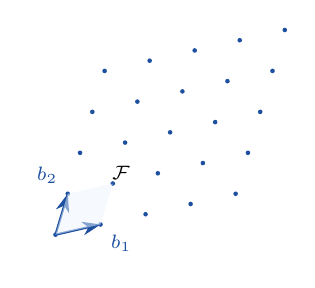
\begin{tikzpicture}[scale=0.52]
        \foreach \i in {0,...,4}\foreach \j in {0,...,4}
          \fill[accent] ($\i*(1.1,0.25)+\j*(0.3,1.0)$) circle (1.6pt);
        \draw[-{Stealth}, accent, thick] (0,0)--(1.1,0.25) node[below right]{\scriptsize$b_1$};
        \draw[-{Stealth}, accent, thick] (0,0)--(0.3,1.0) node[above left]{\scriptsize$b_2$};
        \fill[accentlt, opacity=0.5] (0,0)--(1.1,0.25)--(1.4,1.25)--(0.3,1.0)--cycle;
        \node[font=\scriptsize] at (1.6,1.5) {$\mathcal{F}$};
      \end{tikzpicture}
    \end{column}
  \end{columns}
\end{frame}

% ── Minkowski ──
\begin{frame}{Minkowski 第一定理（1896）}{Part 0 · 預備概念 2/6}
  \begin{block}{定理}
    設 $\mathcal{L}\subset\R^n$ 為格，$S\subset\R^n$ 為\textbf{中心對稱凸體}
    （$x\in S\Rightarrow -x\in S$，有界閉凸）。若
    \[
      \vol(S) > 2^n \det(\mathcal{L}),
    \]
    則 $S$ 含至少一個非零格點 $v\in\mathcal{L}\setminus\{0\}$。
  \end{block}
  \begin{itemize}\small
    \item \textbf{證明構想}：對 $\tfrac12 S$ 套用 Blichfeldt 鴿巢論證，
      $\vol(\tfrac12 S)>\det(\mathcal{L})$ 迫使兩平移拷貝重疊，
      再用中心對稱 $+$ 凸性把差向量拉回 $S$。
    \item \textbf{核心訊息}：「體積夠大 $\Rightarrow$ 非零格點必存在」——
      一個\textbf{非構造性}存在定理：保證短向量\emph{存在}，卻不給尋找方法。
    \item 這正是 SVP 困難性的幾何根源，也是格密碼安全性的基石。
  \end{itemize}
\end{frame}

% ── 分圓域 ──
\begin{frame}{分圓域（Cyclotomic Field）}{Part 0 · 預備概念 3/6}
  \begin{block}{設定（取 $n=2^k$，二的冪分圓環）}
    $\zeta=\zeta_{2n}=e^{i\pi/n}$ 為第 $2n$ 個本原單位根，分圓多項式
    $\Phi_{2n}(x)=x^n+1$（$n=2^k$ 時於 $\Q$ 上不可約），
    $K=\Q(\zeta)$，$[K:\Q]=n$。
  \end{block}
  \begin{itemize}\small
    \item 整數環 $\OK=\Z[\zeta]\cong\Z[x]/(x^n+1)$ 為 \textbf{Dedekind 整環}
      （Noetherian、整閉、非零質理想皆極大）$\Rightarrow$ 每個非零理想有唯一質理想積分解。
    \item \textbf{標準嵌入} $\sigma_j(\zeta)=\zeta^{2j-1}$（$j=1,\dots,n$）給出
      $\sigma:K\hookrightarrow\mathbb{C}^n$；共軛對稱使像落在 $H\cong\R^n$ 中，
      且與環乘法相容（逐分量乘法）。
    \item 判別式 $|\Delta_K|=(2n)^n/2^n=n^n$。
    \item 選 $x^n+1$ 的理由：不可約性最簡、$x^n\equiv-1$ 帶來「負循環卷積」、利於 NTT。
  \end{itemize}
\end{frame}

% ── 理想格結構 ──
\begin{frame}{理想格結構（Ideal Lattice）}{Part 0 · 預備概念 4/6}
  \begin{block}{理想 $\xrightarrow{\ \sigma\ }$ 格}
    分式理想 $\mathfrak{a}\subset\OK$ 透過標準嵌入給出 $\sigma(\mathfrak{a})\subset H$，
    為秩 $n$ 的格，且在 $\OK$ 的乘法作用下封閉（故稱\textbf{理想格}）。
  \end{block}
  \begin{itemize}\small
    \item 覆積與理想範數 $N(\mathfrak{a})=[\OK:\mathfrak{a}]$ 的精確關係：
      \[
        \det\bigl(\sigma(\OK)\bigr)=\sqrt{|\Delta_K|}=n^{n/2},
        \qquad
        \det\bigl(\sigma(\mathfrak{a})\bigr)=N(\mathfrak{a})\cdot n^{n/2}.
      \]
    \item \textbf{意義}：把「理想範數」（算術量）與「格體積」（幾何量）綁定；
      理想乘法 $\leftrightarrow$ 格的代數作用。
    \item 理想格只是「一般格」的特例，但帶有額外環結構 $\Rightarrow$
      \alert{效率提升的根源}（Ring-LWE），同時也是\alert{安全爭議的來源}（Ideal-SVP 是否較易）。
  \end{itemize}
\end{frame}

% ── SVP ──
\begin{frame}{最短向量問題 SVP（Shortest Vector Problem）}{Part 0 · 預備概念 5/6}
  \begin{columns}[T]
    \begin{column}{0.62\textwidth}
      \begin{block}{問題}
        給定格 $\mathcal{L}$ 的（壞）基底，求最短非零向量長度
        $\lambda_1(\mathcal{L})=\min_{v\in\mathcal{L}\setminus\{0\}}\|v\|$，
        或求達此長度的 $v$。
      \end{block}
      \begin{itemize}\small
        \item \textbf{近似版 SVP$_\gamma$}：找 $v\neq0$ 使 $\|v\|\le\gamma\cdot\lambda_1$。
        \item NP-hard（隨機歸約，$\gamma=O(1)$）；最佳演算法 $2^{\Theta(n)}$。
        \item 最佳量子演算法 $2^{0.265n}$（Laarhoven 2015）$\Rightarrow$ 後量子仍困難。
        \item LWE/Ring-LWE 的安全性最終歸約至此（worst-case）。
      \end{itemize}
    \end{column}
    \begin{column}{0.36\textwidth}
      \centering
      \begin{tikzpicture}[scale=0.5]
        \foreach \i in {-1,...,3}\foreach \j in {-1,...,3}
          \fill[gray!60] ($\i*(1.2,0.3)+\j*(0.4,1.1)$) circle (1.4pt);
        \draw[-{Stealth}, warn, very thick] (0,0)--(0.4,1.1);
        \node[warn, font=\scriptsize] at (1.1,1.0) {最短 $v$};
      \end{tikzpicture}
      \\[2pt]{\scriptsize 求最短的非零格點}
    \end{column}
  \end{columns}
\end{frame}

% ── CVP ──
\begin{frame}{最近向量問題 CVP（Closest Vector Problem）}{Part 0 · 預備概念 6/6}
  \begin{columns}[T]
    \begin{column}{0.62\textwidth}
      \begin{block}{問題}
        給定格 $\mathcal{L}$ 與目標點 $t\in\R^n$（不一定在格上），
        求最近格點 $v\in\mathcal{L}$ 使 $\|t-v\|$ 最小。
      \end{block}
      \begin{itemize}\small
        \item 一般比 SVP 更難（SVP $\le$ CVP 可歸約）。
        \item \textbf{BDD（Bounded Distance Decoding）}：CVP 的特例，
          已知 $t$ 距某格點極近（$<\lambda_1/2$），求該格點 $\Rightarrow$ 解唯一。
        \item \alert{LWE 的本質就是 BDD}：$b=As+e$ 中 $As$ 是格點、$e$ 是小誤差，
          還原 $s$ $=$ 在 $q$-ary 格上解 BDD。
      \end{itemize}
    \end{column}
    \begin{column}{0.36\textwidth}
      \centering
      \begin{tikzpicture}[scale=0.5]
        \foreach \i in {-1,...,3}\foreach \j in {-1,...,3}
          \fill[gray!60] ($\i*(1.2,0.3)+\j*(0.4,1.1)$) circle (1.4pt);
        \coordinate (t) at (1.7,1.6);
        \coordinate (v) at (1.6,1.4);
        \fill[warn] (t) circle (2pt) node[right, font=\scriptsize]{$t$};
        \draw[warn, thick, dashed] (t)--(v);
        \fill[accent] (v) circle (2pt) node[below, font=\scriptsize]{$v$};
      \end{tikzpicture}
      \\[2pt]{\scriptsize 求離 $t$ 最近的格點}
    \end{column}
  \end{columns}
\end{frame}

% ══════════════════════════════════════════════════════════
\section{Part 1 — LWE（重點）}

\begin{frame}{LWE：問題設定（Regev 2005）}{Part 1 · 重點}
  \begin{block}{Learning With Errors}
    固定維度 $n$、模數 $q$、誤差分布 $\chi$（寬度 $\alpha q$ 的離散高斯，$\alpha\ll1$）。
    秘密 $s\in\Z_q^n$。每筆樣本：
    \[
      a \xleftarrow{\$} \Z_q^n,\qquad
      b = \langle a, s\rangle + e \bmod q,\quad e\leftarrow\chi.
    \]
  \end{block}
  \begin{itemize}\small
    \item 收集 $m$ 筆寫成矩陣形式：$A\in\Z_q^{m\times n}$，
      \[
        b = A s + e \bmod q \in \Z_q^m.
      \]
    \item 直覺：若無誤差 $e$，由 $n$ 條線性方程即可高斯消去解出 $s$；
      \alert{加入微小誤差後，線性代數失效}——這正是困難所在。
    \item 誤差 $e$ 必須「夠小以保正確性、夠大以保安全性」，由 $\alpha$ 調控。
  \end{itemize}
\end{frame}

\begin{frame}{LWE：判定版本與搜尋版本}{Part 1 · 重點}
  \begin{columns}[T]
    \begin{column}{0.5\textwidth}
      \begin{block}{Search-LWE}
        給定多筆 $(a_i,b_i)$，\textbf{還原秘密 $s$}。
      \end{block}
    \end{column}
    \begin{column}{0.5\textwidth}
      \begin{block}{Decision-LWE}
        區分以下兩種分布：\\
        $(a, \langle a,s\rangle+e)$ \quad vs.\quad
        $(a, u)$，$u\xleftarrow{\$}\Z_q$ 均勻。
      \end{block}
    \end{column}
  \end{columns}
  \vspace{4pt}
  \begin{itemize}\small
    \item 兩者\textbf{多項式時間等價}（search-to-decision，質數 $q$ 時 Regev 給出歸約）。
    \item \textbf{加密應用以 Decision 版為基礎}：密文與隨機串不可區分 $\Rightarrow$ 語意安全（IND-CPA）。
    \item 範例（Regev 加密）：公鑰 $(A, b=As+e)$；加密位元 $\mu$ 取子集和
      $\bigl(\textstyle\sum a_i,\ \sum b_i + \mu\lfloor q/2\rfloor\bigr)$，
      解密看內積是否接近 $0$ 或 $q/2$。
  \end{itemize}
\end{frame}

\begin{frame}{LWE：與格的連結與安全歸約}{Part 1 · 重點}
  \begin{block}{$q$-ary 格上的 BDD}
    令 $\Lambda_q(A)=\{y\in\Z^m: y\equiv As \bmod q,\ \exists s\in\Z_q^n\}$。
    則 $b=As+e$ 是\textbf{靠近格點 $As$ 的目標點}，誤差 $e$ 即偏移量
    $\Rightarrow$ 還原 $s$ $=$ 在 $\Lambda_q(A)$ 上解 \textbf{BDD/CVP}。
  \end{block}
  \begin{block}{Regev 量子歸約（worst-case $\to$ average-case）}
    \[
      \text{worst-case GapSVP}_\gamma \,/\, \text{SIVP}_\gamma
      \;\xrightarrow{\ \text{量子多項式時間}\ }\;
      \text{average-case LWE},\quad \gamma=\tilde{O}(n/\alpha).
    \]
  \end{block}
  \begin{itemize}\small
    \item 意義：\alert{破解隨機 LWE 實例} $\Rightarrow$ \alert{解最壞情況格問題}——
      安全性建立在「最難實例」之上。
    \item Peikert（2009）後補古典歸約（針對 GapSVP、大 $q$）。
  \end{itemize}
\end{frame}

\begin{frame}{LWE：困難性與效率瓶頸}{Part 1 · 重點 — 承接 Ring-LWE 的動機}
  \begin{itemize}\small
    \item \textbf{優點}：安全性歸約乾淨、無額外代數結構假設 $\Rightarrow$ 最保守的格密碼基礎。
    \item \textbf{致命瓶頸（效率）}：
      \begin{itemize}
        \item 公鑰是 $m\times n$ 矩陣 $A$ $\Rightarrow$ 大小 $O(n^2)$（甚至 $\tilde O(n^2)$）。
        \item 每次運算為一般矩陣–向量乘 $\Rightarrow$ $O(n^2)$ 時間。
        \item 為達實用安全（$n\sim10^3$），金鑰動輒數 MB，難以部署。
      \end{itemize}
  \end{itemize}
  \begin{block}{核心問題}
    能否在\textbf{不犧牲安全歸約}的前提下，把 $O(n^2)$ 降到接近線性？\\
    \alert{解法：賦予秘密與樣本「環結構」} $\Rightarrow$ 一個環元素 $a\in R_q$
    一次給出 $n$ 條方程，金鑰 $O(n)$、乘法 $O(n\log n)$。\quad
    這就是 \textbf{Ring-LWE}。
  \end{block}
\end{frame}

% ══════════════════════════════════════════════════════════
\section{Part 2 — Ring-LWE（重點）}

\begin{frame}{Ring-LWE：分圓環設定（LPR 2010）}{Part 2 · 重點}
  \begin{block}{環的設定}
    $R=\OK=\Z[x]/(x^n+1)$（$n=2^k$），$R_q=R/qR\cong\Z_q[x]/(x^n+1)$。
    秘密 $s\in R_q$，誤差 $e\leftarrow\chi_R$（$R$ 上窄離散高斯）。樣本：
    \[
      a \xleftarrow{\$} R_q,\qquad b = a\cdot s + e \in R_q.
    \]
  \end{block}
  \begin{itemize}\small
    \item 對照 LWE：向量 $\Z_q^n$ $\to$ 環元素 $R_q$；內積 $\to$ \textbf{環乘法}（負循環卷積）。
    \item 單一 $a\in R_q$（$n$ 個係數）即攜帶 $n$ 條「方程」$\Rightarrow$ 金鑰由 $O(n^2)$ 降為 $O(n)$。
    \item 安全性歸約至\textbf{理想格}上的 ideal-SVP（而非任意格）。
    \item 代數結構（質理想分解、CRT、對偶格）使運算可加速、歸約可成立。
  \end{itemize}
\end{frame}

\begin{frame}{Ring-LWE：質理想分解與 $R_q\cong\F_q^n$}{Part 2 · 重點}
  對質數 $q\nmid 2n$，$q$ 在 $\OK$ 的分解由 $\Phi_{2n}(x)\bmod q$ 的因式分解決定：
  \[
    \Phi_{2n}(x)\equiv\prod_{i=1}^{g}\phi_i(x)^{e_i}\!\!\pmod q,\quad \deg\phi_i=f,\ \ efg=n,
    \qquad q\OK=\mathfrak{q}_1^{e_1}\cdots\mathfrak{q}_g^{e_g}.
  \]
  \begin{block}{完全分裂條件}
    $q$ 完全分裂（$e=f=1,\ g=n$）$\iff q\equiv1\pmod{2n}$。
    此時 $\F_q^\times$ 含 $2n$ 次本原單位根 $\omega$，
    $\Phi_{2n}(x)\equiv\prod_{j=1}^n(x-\omega_j)\pmod q$，由 CRT：
    \[
      R_q\;\xrightarrow{\ \cong\ }\;\prod_{j=1}^n \F_q[x]/(x-\omega_j)\;\cong\;\F_q^n,
      \qquad a(x)\mapsto\bigl(a(\omega_1),\dots,a(\omega_n)\bigr).
    \]
  \end{block}
  \begin{itemize}\small
    \item 環同構把\textbf{多項式乘法}化為 $\F_q^n$ 中的\textbf{逐分量乘法}——下一頁 NTT 的代數根源。
    \item 故參數恆取 $q\equiv1\pmod{2n}$。
  \end{itemize}
\end{frame}

\begin{frame}{Ring-LWE：NTT — 環乘法的 $O(n\log n)$ 運算}{Part 2 · 重點}
  \begin{block}{數論變換 NTT}
    完全分裂下定義求值映射
    $\widehat{a}=\mathrm{NTT}(a):=(a(\omega_1),\dots,a(\omega_n))\in\F_q^n$，則
    \[
      \mathrm{NTT}(a\cdot b)=\mathrm{NTT}(a)\odot\mathrm{NTT}(b)
      =\bigl(a(\omega_j)\,b(\omega_j)\bigr)_{j=1}^n,
    \]
    乘完以反變換 $\mathrm{NTT}^{-1}$（插值，含 $n^{-1}\bmod q$ 縮放）取回係數。
  \end{block}
  \begin{itemize}\small
    \item \textbf{Cooley–Tukey 蝴蝶}：依奇偶指標遞迴拆解，
      $a(\omega_j)=a_{\text{even}}(\omega_j^2)+\omega_j\,a_{\text{odd}}(\omega_j^2)$，
      配合 $\omega^n=-1$，得 $T(n)=2T(n/2)+O(n)=O(n\log n)$。
    \item $x^n+1\Rightarrow x^n\equiv-1$，環乘法即\textbf{負循環卷積}
      （繞回項變號）——選二的冪分圓環以簡化此運算。
    \item 效率對照：直接多項式乘法 $O(n^2)$ \ $\to$\ NTT $O(n\log n)$。
  \end{itemize}
\end{frame}

\begin{frame}{Ring-LWE：對偶格與誤差的自然定義域}{Part 2 · 重點}
  \begin{block}{差異理想與逆差理想（對偶格）}
    差異理想 $\mathfrak{D}_{K/\Q}=(\Phi_{2n}'(\zeta))=(n\zeta^{n-1})=(n)$；
    跡配對 $\langle a,b\rangle=\Tr_{K/\Q}(ab)$ 下，$\OK$ 的\textbf{對偶格}為逆差理想
    \[
      \mathfrak{D}^{-1}=\{x\in K:\Tr_{K/\Q}(x\,\OK)\subset\Z\}=\tfrac1n\OK.
    \]
  \end{block}
  \begin{itemize}\small
    \item 驗證關鍵：$\Tr_{K/\Q}(\zeta^j)=n$（$j=0$）或 $0$（$1\le j\le n-1$）。
    \item \textbf{密碼學意義}：嚴格 Ring-LWE 中誤差定義於
      $\mathfrak{D}^{-1}/q\mathfrak{D}^{-1}=\tfrac1n R_q$（非 $R_q$ 本身），
      唯有對偶格才能讓誤差分布在跡配對下保持\textbf{代數不變性}，確保歸約嚴密。
    \item 二的冪分圓環因 $\mathfrak{D}=(n)$ 為主理想，此修正僅是 $\tfrac1n$ 縮放，實作簡潔。
  \end{itemize}
\end{frame}

\begin{frame}{Ring-LWE：歸約鏈與 LWE 對照}{Part 2 · 重點 — 小結}
  \begin{block}{安全歸約鏈（量子，LPR 2010）}
    \[
      \text{worst-case ideal-SVP}_\gamma
      \xrightarrow{\ \text{量子多項式}\ }
      \text{average-case Ring-LWE}
      \Longrightarrow
      \text{破解 Kyber/Dilithium 困難}.
    \]
  \end{block}
  \begin{center}\small
  \begin{tabular}{l c c c}
    \hline
    & 金鑰大小 & 乘法成本 & 安全基礎 \\
    \hline
    LWE（Regev 2005） & $O(n^2)$ & $O(n^2)$ 矩陣乘 & 任意格 SVP/SIVP \\
    Ring-LWE（LPR 2010） & $O(n)$ & $O(n\log n)$ NTT & 理想格 ideal-SVP \\
    \hline
  \end{tabular}
  \end{center}
  \vspace{2pt}
  \begin{itemize}\small
    \item 代數結構（分圓環、CRT、NTT、對偶格）讓 Ring-LWE
      \alert{在維持與 LWE 相近的安全保證下，把成本由 $O(n^2)$ 壓到 $O(n\log n)$}。
    \item 代價：安全性多依賴「理想格」假設（見開放問題）。
  \end{itemize}
\end{frame}

% ══════════════════════════════════════════════════════════
\section{Part 3 — 應用與開放問題}

\begin{frame}{應用：NIST 後量子標準（2024.08）}{Part 3 · 約 5 分}
  \begin{itemize}\small
    \item \textbf{FIPS 203（ML-KEM = Kyber）}：金鑰封裝，基於 \textbf{Module-LWE}
      （Ring-LWE 在模組格 $R_q^{k\times k}$ 上的推廣）；
      Kyber-512 取 $n=256$、$q=3329$，NIST Level I（攻擊難度 $\approx2^{118}$）。
    \item \textbf{FIPS 204（ML-DSA = Dilithium）}：數位簽章，基於 Module-LWE $+$ Module-SIS；
      公鑰約 1.3 KB、簽章約 2.4 KB。
    \item Module-LWE 折衷：介於 Ring-LWE（最快、結構最多）與 LWE（最保守）之間，
      以小矩陣 $k\times k$ 換取「降結構風險 $+$ 仍可用 NTT」。
  \end{itemize}
  \begin{block}{安全鏈}
    \[
      \text{破解密碼} \iff \text{解 BDD on ideal lattice} \impliedby \text{ideal-SVP}_\gamma\ \text{困難}.
    \]
  \end{block}
\end{frame}

\begin{frame}{開放問題}{Part 3 · 約 5 分}
  \begin{itemize}\small
    \item \textbf{Ideal-SVP vs SVP}：理想格的 SVP 是否真不比任意格容易？
      Cramer et al.（2016）對特定分圓環給出量子加速；一般情形仍開放。
      若 ideal-SVP 易解，Ring-LWE 安全保證將弱化。
    \item \textbf{非分圓域的 Ring-LWE}：LPR 歸約依賴分圓域的交換 Galois 結構；
      對 Galois 閉包為非交換群的數環，歸約是否成立未知。
    \item \textbf{古典 worst-case 歸約}：Regev 的 LWE 歸約為量子的；
      純古典 worst-case $\to$ average-case 歸約至今未尋得。
    \item \textbf{SVP 量子下界}：最佳量子演算法 $2^{0.265n}$（Laarhoven 2015），
      無條件指數下界至今未被證明。
  \end{itemize}
\end{frame}

\begin{frame}[plain]{}{}
  \vfill
  \begin{center}
    {\Large\bfseries\color{accent} 謝謝聆聽}\\[6pt]
    {\small\color{gray} 提問與討論}
  \end{center}
  \vfill
  \begin{center}\scriptsize\color{gray}
    O.\ Regev, \textit{J.\ ACM} \textbf{56}(6), 2009.\quad
    V.\ Lyubashevsky--C.\ Peikert--O.\ Regev, \textit{J.\ ACM} \textbf{60}(6), 2013.\\
    H.\ Minkowski, \textit{Geometrie der Zahlen}, 1896.\quad
    J.\ Neukirch, \textit{Algebraic Number Theory}, Springer, 1999.\quad
    NIST FIPS 203/204, 2024.\\[4pt]
    延伸參考（整理來源）：\\
    \url{https://hackmd.io/9wQpRveaS4ywg2XBugxF0A}\\
    \url{https://drive.google.com/file/d/1OdtsrpwJK5mDYlakeiCoA-2uOmbF9ydp/view?pli=1}
  \end{center}
\end{frame}

\end{document}
